\documentclass{beamer}
\usetheme{CambridgeUS}
\usepackage[utf8]{inputenc}
\usepackage{tikz}
\usetikzlibrary{quotes} % LATEX and plain TEX



\title{1-2-3 Domneva}

\author{Gašper Domen Romih}

\date{\today}

\begin{document}
\begin{frame}
	\titlepage
\end{frame}
\begin{frame}
\tableofcontents
\end{frame}
\section{Osnovne definicije}

\begin{frame}
\begin{block}{Graf}
Graf $G$ je urejen par $(V, E)$, kjer je množica $V$ množice vozlišč in $E \subset V^2$ množice povezav.
\end{block}

\begin{block}{Barvanje grafa}
	Barvanje grafa $G = (V, E)$ je preslikava $c : V \rightarrow S$. Množici $S$ rečemo množica barv. Rečemo, da je barvanje \textbf{pravilno}, če za vsak $uv \in E$ velja $c(u) \neq c(v)$.
\end{block}
\begin{block}{Utežitev grafa}
	Utežitev grafa je preslikava $\omega : E \rightarrow W$. V kolikor je množica uteži $W$ oblike $\{1,2,\ldots, k\}$ rečemo, da je preslikava $\omega$ $k$-utežitev grafa $G$.
\end{block}
\end{frame}

\begin{frame}{Od utežitve do barvanja}
\begin{block}{Barvanje grafa z $k$-utežitvijo}
	Naj bo $\omega$ neka $k$-utežitev grafa $G$. Sedaj definiramo preslikavo $c_{\omega} : V \rightarrow S$ na naslednji način:
	$$ c_{\omega}(u) = \sum_{e = uv \in E} \omega(e). $$
\end{block}
\begin{figure}
			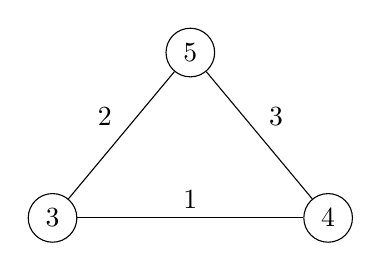
\begin{tikzpicture}
	[scale=.7,auto=left,main node/.style={shape=circle,draw,fill=white}]
	\node [main node] (1) at (0,0) {3};
	\node [main node] (2) at (5,0) {4};
	\node [main node] (3) at (2.5,3) {5};
	
	
	\path[]
	(1) edge node {1} (2)
	(1) edge node {2} (3)
	(2) edge node [above right] {3} (3)
	
	;
	
	
	
	\end{tikzpicture}
	\caption{Primer $3$-utežitve, ki porodi pravilno $3$-barvanje.}
\end{figure}

\end{frame}

\section{1-2-3 Domneva}
\begin{frame}
\begin{block}{}
	Označimo z $\mu(G)$ najmanjši tak $k$ za katerega obstaja $k$-utežitev $\omega$ grafa $G$, ki inducira pravilno barvanje $c_{\omega}$.
\end{block}
\begin{block}{1-2-3 Domneva}
	Za vsak povezan graf $G$, ki ni $K_2$ je $\mu(G) \le 3$.
\end{block}
\end{frame}

\subsection{Zgodovinski okvir}
\begin{frame}
\begin{itemize}
	\item Leta 2004 v članku [] zastavljena domneva.
	\item Leta 2007 dokazano $\mu(G) \le 30$.
	\item Leta 2008 dokazano $\mu(G) \le 16$.
	\item Leta 2008 dokazano $\mu(G) \le 13$.
	\item Leta 2009 $\mu(G) \le 6$.
	\item Leta 2010 $\mu(G) \le 5$. To je do sedaj tudi najboljši rezultat za splošne grafe.
\end{itemize}

\begin{block}{Opomba}
	Kljub temu, da je trenutno najboljša zgornja $\mu(G) \le 5$ je veliko znaninh družin grafov dokazano $\mu(G) \le 3$.
\end{block}
\end{frame}





\end{document}